\documentclass[3p,11pt,authoryear]{elsarticle}  %preprint, 1p/3p/5p journal
\usepackage{setspace}
\onehalfspacing

\usepackage[utf8]{inputenc}

% --- Bibliography ---

\usepackage{natbib}
%\usepackage{natbib}
%\bibpunct[, ]{(}{)}{,}{a}{}{,}%
% \def\bibfont{\small}%
% \def\bibsep{\smallskipamount}%
% \def\bibhang{24pt}%
% \def\newblock{\ }%
% \def\BIBand{and}%

\usepackage{hyperref}
%% APA style
\bibliographystyle{model5-names-new}   %model5-names, unsrt, apalike, plainnat
%plainnat works. But there is an error somewhere in the bibliography for the other styles

\usepackage{comment}

\RequirePackage{tgtermes}
\RequirePackage{newtxtext}
\RequirePackage{newtxmath}
\RequirePackage{bm}
\RequirePackage{endnotes}
\usepackage{changepage} % for adjustwidth
\usepackage{booktabs}
\usepackage{threeparttable}
\usepackage{siunitx}
\usepackage{amsmath} % for adjustwidth
\usepackage{makecell}
\usepackage{xcolor}
\usepackage{subcaption}
% Define the custom command
\newcommand{\red}[1]{{\textcolor{red}{#1}}}
%\OneAndAHalfSpacedXI
\usepackage{algorithm}
\usepackage{algpseudocode}
\usepackage{tikz}
% Private macros here (check that there is no clash with the style)
\usepackage{graphicx}
\usetikzlibrary{arrows.meta,positioning,decorations.pathreplacing,shapes.geometric}
% Natbib setup for author-number style
\usepackage{longtable}
\usepackage{multirow}
\usepackage{multicol}
\usepackage{makecell}
\journal{Transportation Research Part E: Logistics and Transportation Review}


%%%%%%%%%%%%%%%%
\begin{document}

%%%%%%%%%%%%%%%%

%------------------------------------------------%

\section{SPPRC Framework} 

%------------------------------------------------%

The EVTDSP can be formulated as a shortest path problem with resource constraints (SPPRC) and solved using a labeling algorithm. Our modeling approach extends the parameter-free network and labeling framework of \citet{goel2017exact} to account for battery-electric truck operations. Feasibility is tracked through label resources representing elapsed time, Hours-of-Service counters, and battery-energy state. These resources are propagated through the network by resource extension functions (REFs) associated with the network arcs. We present the partial-recharge strategy, in which charging amounts are decision variables. The full-recharge strategy is obtained as a special case in which each charging action restores the battery to full capacity; the corresponding network details are reported in Appendix~\ref{app:full_recharge_spprc}. The remainder of this section first presents the underlying activity network, then introduces the label resources and REFs, and finally describes the feasibility and dominance rules used within the labeling algorithm.

%------------------------------------------------%

\subsection{Parameter-free network structure}

%------------------------------------------------%

Charging stations are introduced as additional physical nodes along the route, so that a leg between two mandatory locations may be decomposed into several consecutive sublegs. Figure~\ref{fig:subnetwork_cs_partial} illustrates a route segment from customer $n$ to customer $m$ with an intermediate charging station $s$, resulting in the sublegs $(n,s)$ and $(s,m)$.

\begin{figure}[htbp!]
\centering
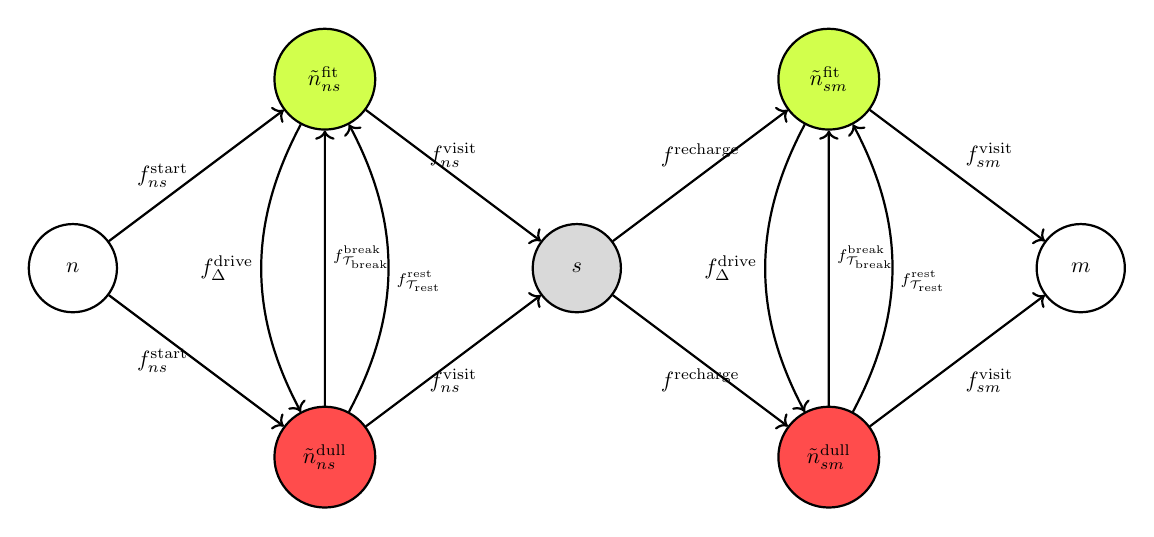
\begin{tikzpicture}[scale=0.8, transform shape, ->, thick, auto]
% Node styles
\tikzstyle{main} = [circle, draw=black, minimum size=1.4cm, inner sep=0pt]
\tikzstyle{fit}  = [circle, draw=black, fill=lime!70, minimum size=1.6cm, inner sep=0pt]
\tikzstyle{dull} = [circle, draw=black, fill=red!70, minimum size=1.6cm, inner sep=0pt]
\tikzstyle{cs}   = [circle, draw=black, fill=gray!30, minimum size=1.4cm, inner sep=0pt]

% Nodes
\node[main] (n) at (0,0) {$n$};
\node[fit]  (fitL) at (4, 3) {$\tilde{n}^{\text{fit}}_{ns}$};
\node[dull] (dullL) at (4, -3) {$\tilde{n}^{\text{dull}}_{ns}$};
\node[cs]   (cs) at (8, 0) {$s$};
\node[fit]  (fitR) at (12, 3) {$\tilde{n}^{\text{fit}}_{sm}$};
\node[dull] (dullR) at (12, -3) {$\tilde{n}^{\text{dull}}_{sm}$};
\node[main] (m) at (16,0) {$m$};

% From n to left states
\path (n) edge node[left] {$f^{\text{start}}_{ns}$} (fitL);
\path (n) edge node[left] {$f^{\text{start}}_{ns}$} (dullL);

% Transitions between fit/dull (left side)
\path[bend right=28] (fitL) edge node[left] {$f^{\text{drive}}_{\Delta}$} (dullL);
\path (dullL) edge node[right, yshift=5pt] {\scriptsize $f^{\text{break}}_{\mathcal{T}_{\text{break}}}$} (fitL);
\path[bend right=28] (dullL) edge node[right, yshift=-6pt] {\scriptsize $f^{\text{rest}}_{\mathcal{T}_{\text{rest}}}$} (fitL);

% To s
\path (fitL) edge node[above] {$f^{\text{visit}}_{ns}$} (cs);
\path (dullL) edge node[below] {$f^{\text{visit}}_{ns}$} (cs);

% From s to right states
\path (cs) edge node[above] {$f^{\text{recharge}}$} (fitR);
\path (cs) edge node[below] {$f^{\text{recharge}}$} (dullR);

% Transitions between fit/dull (right side)
\path[bend right=28] (fitR) edge node[left] {$f^{\text{drive}}_{\Delta}$} (dullR);
\path (dullR) edge node[right, yshift=5pt] {\scriptsize $f^{\text{break}}_{\mathcal{T}_{\text{break}}}$} (fitR);
\path[bend right=28] (dullR) edge node[right, yshift=-6pt] {\scriptsize $f^{\text{rest}}_{\mathcal{T}_{\text{rest}}}$} (fitR);

% From right states to m
\path (fitR) edge node[above right] {$f^{\text{visit}}_{sm}$}  (m);
\path (dullR) edge node[below right] {$f^{\text{visit}}_{sm}$} (m);
\end{tikzpicture}
\caption{Extended subnetwork with an intermediate charging station $s$ under the partial-recharge strategy.}
\label{fig:subnetwork_cs_partial}
\end{figure}

Each subleg is represented by an activity subnetwork containing two intermediate states, denoted by \(\tilde n_{nm}^{\mathrm{fit}}\) and \(\tilde n_{nm}^{\mathrm{dull}}\). The \emph{fit} state represents a situation in which the driver is allowed to continue driving, either because no break or daily rest is currently due or because the required one has already been completed. The \emph{dull} state represents a situation in which the driver must first take a break or daily rest before additional driving is permitted. Arcs between these states correspond to elementary driver activities, namely starting a leg, driving, taking a break, taking a daily rest, visiting the next physical node, and recharging at a charging station.

At a charging-station node, the schedule may initiate a charging activity. Under the partial-recharge strategy, the amount of energy charged is not fixed in advance. Charging is represented through recharge arcs originating from the charging-station node. These arcs preserve the feasible continuation of both fit and dull driver states while introducing the operational choice of how much energy to recharge.

The resulting network contains six classes of arcs: start arcs, driving arcs, break arcs, rest arcs, visit arcs, and recharge arcs. A key feature of this representation is that a driving arc is not assigned a fixed duration in advance. Instead, its extension length \(\Delta\) is computed dynamically as the largest admissible driving time consistent with the current resource state. \(\Delta\) is the minimum of (i) the remaining travel time to the next physical node, (ii) the remaining driving time until a mandatory break or daily rest, (iii) the remaining daily working time before a mandatory rest must begin, and (iv) the remaining driving time permitted by the available battery energy. Consequently, each driving extension terminates either at the next physical node or at the point where HoS or energy considerations require a new decision.

%------------------------------------------------%

\subsection{Labeling algorithm}

%------------------------------------------------%

The activity network introduced above compactly represents feasible combinations of driving, charging, breaks, and daily rests. Finding an optimal schedule therefore reduces to finding a shortest feasible path through this network. To solve the resulting SPPRC, we employ a labeling algorithm in which each label represents a partial path together with the associated driver and vehicle resource state. Feasible schedules are constructed incrementally through label extension and resource propagation.

The algorithm starts from a single initial label at the origin, corresponding to a fully rested and fully charged vehicle-driver state. At each iteration, an unprocessed label is selected and extended along all outgoing arcs that are feasible with respect to the current resource state. Each extension generates a new label whose temporal, regulatory, and energy-related resources are updated according to the REF of the traversed arc. Labels that violate HoS or battery-feasibility conditions are discarded immediately. Whenever several labels reach the same network node, dominance rules are applied to eliminate labels that cannot lead to a better feasible completion than another label at that node. In this way, the algorithm explores only nondominated partial schedules. A label is complete when it reaches the destination node after all mandatory visits have been performed in the prescribed order. The remainder of this subsection specifies the label definition, the resource extension functions, and the associated feasibility and dominance rules for the partial-recharge strategy.

%------------------------------------------------%

\subsubsection{Label definition}

%------------------------------------------------%

A label \(l\) represents a partial path from the origin to a network node together with the temporal, regulatory, and energy state of the driver--vehicle system required to continue that partial schedule. With partial recharging, the amount charged at a station becomes a decision variable. As a consequence, labels arriving at the same node represent a continuum of feasible time--energy trade-offs. To capture these trade-offs compactly, the time and energy components of the label are represented by intervals. Specifically, we maintain a time interval \([l_{\text{time}}^{\min},l_{\text{time}}^{\max}]\), an energy-deficit interval \([l_{\text{reqEC}}^{\min},l_{\text{reqEC}}^{\max}]\), and a state-of-charge interval \([l_{\text{SOC}}^{\min},l_{\text{SOC}}^{\max}]\).

The resource \(l_{\text{time}}\) records the total time elapsed since departure. The resource \(l_{\text{timeToNext}}\) denotes the remaining driving time to the next physical node and is particularly important for modeling traversal between intermediate fit and dull states; it becomes zero when a customer or charging station has been reached. The counters \(l_{\text{drive|R}}\) and \(l_{\text{drive|B}}\) track accumulated driving time since the last daily rest and since the last break, respectively, while \(l_{\text{elapsed|R}}\) and \(l_{\text{elapsed|B}}\) record the corresponding elapsed working time. In contrast to \citet{goel2017exact}, we explicitly retain the break-specific counters \(l_{\text{drive|B}}\) and \(l_{\text{elapsed|B}}\). In our setting these resources can become binding and are necessary to preserve exact compliance with the EU break rules. Table~\ref{tab:resource_windows_partial} summarizes the corresponding feasibility windows.

\begin{table}[!htbp]
\centering
\caption{Label resources with corresponding resource windows.}
\label{tab:resource_windows_partial}
\begin{tabular}{@{}lll@{}}
\toprule
\textbf{Resource} & \textbf{Description} & \textbf{Feasibility Window} \\
\midrule
$ \text{time} $ & Total time elapsed since start & $  [0, T_{\text{horizon}}] $ \\
$ \text{timeToNext} $ & Remaining driving time to next node & $ [0, t_{nm}] $ \\
$ \text{drive|R} $ & Driving time since last rest & $ [0, t_{\text{drive}|R}] $ \\
$ \text{drive|B} $ & Driving time since last break & $ [0, t_{\text{drive}|B}] $ \\
$ \text{elapsed|R} $ & Elapsed time since last rest & $ [0, t_{\text{elapsed}|R}] $ \\
$ \text{elapsed|B} $ & Elapsed time since last break & $ [0, t_{\text{elapsed}|B}] $ \\
$ \text{reqEC} $ & Required energy since last recharge & $ [0, B] $ \\
\bottomrule
\end{tabular}
\end{table}

The HoS-related counters are propagated exactly as in the parameter-free framework, since regulatory feasibility depends on the temporal evolution of activities rather than on the precise state of charge. A partial-recharge label is therefore written as
\[
\begin{aligned}
l = (&l_{\text{time}}^{\min},\, l_{\text{time}}^{\max},\, l_{\text{timeToNext}},\, 
      l_{\text{drive|R}},\, l_{\text{drive|B}},\\
     &l_{\text{elapsed|R}},\, l_{\text{elapsed|B}}, \\ 
     &l_{\text{reqEC}}^{\min},\, l_{\text{reqEC}}^{\max},
      l_{\text{SOC}}^{\min},\, l_{\text{SOC}}^{\max})
\end{aligned}
\]
Feasibility of each label extension is enforced by requiring all resource components to remain within their prescribed bounds. Under partial recharge, the feasibility bounds in Table~\ref{tab:resource_windows_partial} apply componentwise to the corresponding interval endpoints. The full-recharge strategy is recovered when the time and energy intervals reduce to single values after each charging operation; this scalar-label variant is described in Appendix~\ref{app:full_recharge_spprc}.

%------------------------------------------------%

\subsubsection{Resource extension functions}

%------------------------------------------------%

Each arc \(a\in A\) of the parameter-free network is associated with a resource extension function (REF), which maps a feasible label \(l\) at the tail node of \(a\) to a new label \(l'=f_a(l)\) at its head node. The REFs govern how the temporal, regulatory, and energy-related components of a label evolve when a partial schedule is extended by one elementary activity. 

The common REFs based on the parameter-free framework of \citet{goel2017exact} are \(f^{\text{start}}_{nm}\), \(f^{\text{drive}}_{\Delta}\), \(f^{\text{break}}_{\Delta}\), \(f^{\text{rest}}_{\Delta}\), and \(f^{\text{visit}}_{nm}\). The start REF initializes a new travel subleg by setting the remaining travel time to the next physical node. The drive REF propagates time and HoS counters over a driving period of duration \(\Delta\). The break and rest REFs advance time and reset the corresponding regulatory counters. The visit REF models the service or stop activity at a physical node. The duration \(\Delta\) of a driving extension is determined endogenously from the current resource state. Specifically,
\[
\begin{aligned}
\Delta = \min\Bigl\{\, &
l_{\text{timeToNext}},\,
t_{R}^{\text{drive}} - l_{\text{drive|R}},\,
t_{B}^{\text{drive}} - l_{\text{drive|B}},\\
&
t^{\text{day}} - \bigl(l_{\text{elapsed|R}} + t_{\text{rest}}\bigr)
\Bigr\}.
\end{aligned}
\]
Hence, a driving arc terminates either when the next physical node is reached or when a break, a rest, or the daily working-time limit becomes binding. In the EV setting, the extension is additionally restricted by the driving time permitted by the available battery energy.

Under the partial-recharge strategy, \(f^{\text{recharge}}_{\mathrm{cs}}\) propagates an interval of feasible time--energy outcomes, reflecting the fact that the charging amount is itself a decision variable. A single recharge extension therefore represents all feasible charging durations between the minimum amount required to continue and the maximum amount allowed by the battery capacity and station power. When charging overlaps with a legally admissible break or rest, the corresponding HoS counters are updated consistently so that synchronization between charging and regulatory interruptions is captured directly in the label propagation.

Table~\ref{tab:ref_common_partial} summarizes the resource updates for the common REFs. The partial-recharge extension preserves this structure but replaces the scalar charging update by its interval-valued counterpart.

\begin{table}[!htbp]
\caption{Resource updates for the common REFs.}
\label{tab:ref_common_partial}
\centering
\small
\setlength{\tabcolsep}{4pt}
\renewcommand{\arraystretch}{1.15}
\resizebox{\linewidth}{!}{%
\begin{tabular}{@{}lccccc@{}}
\toprule
\textbf{Resource} 
& \( f^{\text{start}}_{nm} \) 
& \( f^{\text{drive}}_{\Delta} \) 
& \( f^{\text{break}}_{\Delta} \) 
& \( f^{\text{rest}}_{\Delta} \) 
& \( f^{\text{visit}}_{nm} \) \\
\midrule
\( l'_{\text{time}} \) 
& --- 
& \( l_{\text{time}} + \Delta \) 
& \( l_{\text{time}} + t_{\text{break}} \) 
& \( l_{\text{time}} + t_{\text{rest}} \) 
& \( l_{\text{time}} + s_m \) \\

\( l'_{\text{timeToNext}} \) 
& \( t_{nm} \) 
& \( l_{\text{timeToNext}} - \Delta \) 
& --- 
& --- 
& --- \\

\( l'_{\text{drive|R}} \) 
& --- 
& \( l_{\text{drive|R}} + \Delta \) 
& --- 
& 0 
& --- \\

\( l'_{\text{drive|B}} \) 
& --- 
& \( l_{\text{drive|B}} + \Delta \) 
& 0 
& 0 
& --- \\

\( l'_{\text{elapsed|R}} \) 
& --- 
& \( l_{\text{elapsed|R}} + \Delta \) 
& \( l_{\text{elapsed|R}} + t_{\text{break}} \) 
& 0 
& \( l_{\text{elapsed|R}} + s_m \) \\

\( l'_{\text{elapsed|B}} \) 
& --- 
& \( l_{\text{elapsed|B}} + \Delta \) 
& 0 
& 0 
& \( l_{\text{elapsed|B}} + s_m \) \\

\( l'_{\text{reqEC}} \) 
& --- 
& \( l_{\text{reqEC}} + \Delta \cdot \alpha \) 
& --- 
& --- 
& --- \\
\bottomrule
\end{tabular}%
}
\end{table}



%------------------------------------------------%

\subsubsection{Feasibility and dominance}

%------------------------------------------------%

After each resource extension, the resulting label must remain feasible with respect to Hours-of-Service requirements and battery-energy constraints. Labels that violate either set of constraints are discarded, while all remaining labels are retained for further extension. Time feasibility requires that the overall elapsed time remains within the planning horizon. Regulatory feasibility is enforced through the driving- and elapsed-time counters \(l_{\text{drive|R}}\), \(l_{\text{drive|B}}\), \(l_{\text{elapsed|R}}\), and \(l_{\text{elapsed|B}}\), which must remain within their respective Hours-of-Service limits. The total elapsed time \(l_{\text{time}}\) is also required to remain within the planning horizon. These bounds ensure that a label is not only currently feasible, but can also be extended without violating future temporal requirements. Energy feasibility is captured through the accumulated energy requirement since the last recharge and the corresponding state-of-charge interval. Under the partial-recharge strategy, the energy and state-of-charge intervals must remain feasible componentwise. Finally, the network structure itself imposes local feasibility conditions: traversals between fit and dull states are admissible only when the associated regulatory and energy requirements of the corresponding activity are satisfied.

To limit the number of labels carried forward, we apply dominance at each network node. Let \(l_1\) and \(l_2\) be two labels ending at the same node. Under partial recharging, label \(l_1\) can dominate label \(l_2\) only if
\[
l_{\text{timeToNext}}^{(1)} \le l_{\text{timeToNext}}^{(2)}
\]
and its driving and elapsed-time resources are no larger componentwise, that is,
\[
\mathbf{l}_{\text{drive}}^{(1)} \le \mathbf{l}_{\text{drive}}^{(2)}, 
\qquad
\mathbf{l}_{\text{elapsed}}^{(1)} \le \mathbf{l}_{\text{elapsed}}^{(2)},
\]
where
\[
\mathbf{l}_{\text{drive}}
=
\bigl(l_{\text{drive|R}},\,l_{\text{drive|B}}\bigr),
\qquad
\mathbf{l}_{\text{elapsed}}
=
\bigl(l_{\text{elapsed|R}},\,l_{\text{elapsed|B}}\bigr).
\]

Because charging couples departure time and energy, dominance also requires the feasible time--energy trade-off represented by \(l_1\) to be nowhere worse than that of \(l_2\) over their comparable departure times. Equivalently, the feasible energy-deficit profile of \(l_1\), which decreases piecewise linearly with charging time until reaching \(l_{\text{reqEC}}^{\min,(1)}\), must lie weakly below the corresponding profile of \(l_2\). In particular, this requires
\[
l_{\text{time}}^{\min,(1)} \le l_{\text{time}}^{\min,(2)},
\qquad
l_{\text{reqEC}}^{\min,(1)} \le l_{\text{reqEC}}^{\min,(2)},
\qquad
l_{\text{reqEC}}^{\max,(1)} \le l_{\text{reqEC}}^{\max,(2)}.
\]
Thus, a single label represents a family of consistent time--charging trade-offs rather than a single point in time--energy space.

Two dominance properties are particularly important. First, break and rest periods should be scheduled at their minimum admissible durations unless extended to synchronize with charging. Second, labels generated by inserting an unnecessary rest or break before an otherwise feasible continuation can be pruned when the resulting label is dominated by one that omits the redundant interruption. When \(\bigl[l_{\text{time}}^{\min},\, l_{\text{time}}^{\max}\bigr]\) reduces to a single time value and \(\bigl[l_{\text{reqEC}}^{\min},\, l_{\text{reqEC}}^{\max}\bigr]\) reduces to a single energy value, these conditions simplify to the scalar full-recharge dominance rule reported in Appendix~\ref{app:full_recharge_spprc}.


%------------------------------------------------%

\section{Full-recharge SPPRC variant and pass-by arcs}
\label{app:full_recharge_spprc}

%------------------------------------------------%

This appendix presents the full-recharge variant of the SPPRC framework. The full-recharge strategy is recovered from the partial-recharge model by restricting every charging action to restore the battery to full capacity. Under this restriction, the energy state can be represented by a scalar resource, and additional pass-by arcs are used to preserve feasible continuations when a charging station is traversed without stopping.

%------------------------------------------------%

\subsection{Network structure with pass-by arcs}

%------------------------------------------------%

Figure~\ref{fig:subnetwork_cs_full} illustrates the extended subnetwork for a route segment from customer \(n\) to customer \(m\) with a single intermediate charging station \(s\). The corresponding sublegs are \((n,s)\) and \((s,m)\).

\begin{figure}[htbp!]
\centering
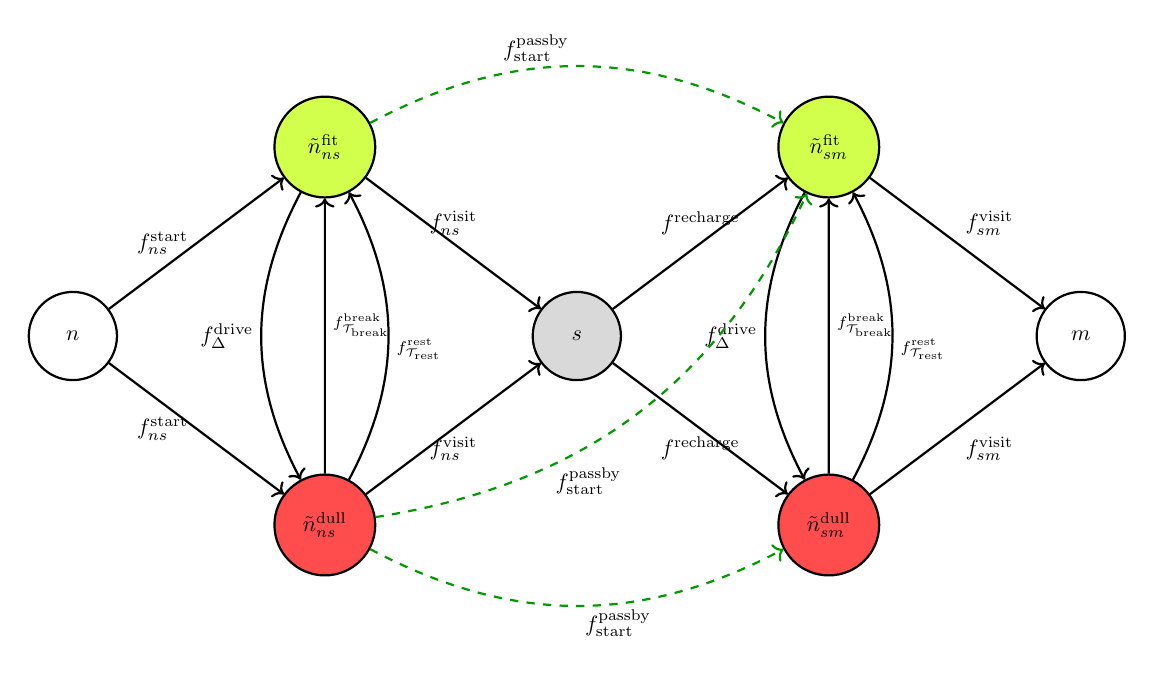
\begin{tikzpicture}[scale=0.8, transform shape, ->, thick, auto]
% Node styles
\tikzstyle{main} = [circle, draw=black, minimum size=1.4cm, inner sep=0pt]
\tikzstyle{fit}  = [circle, draw=black, fill=lime!70, minimum size=1.6cm, inner sep=0pt]
\tikzstyle{dull} = [circle, draw=black, fill=red!70, minimum size=1.6cm, inner sep=0pt]
\tikzstyle{cs}   = [circle, draw=black, fill=gray!30, minimum size=1.4cm, inner sep=0pt]

% Nodes
\node[main] (n) at (0,0) {$n$};
\node[fit]  (fitL) at (4, 3) {$\tilde{n}^{\text{fit}}_{ns}$};
\node[dull] (dullL) at (4, -3) {$\tilde{n}^{\text{dull}}_{ns}$};
\node[cs]   (cs) at (8, 0) {$s$};
\node[fit]  (fitR) at (12, 3) {$\tilde{n}^{\text{fit}}_{sm}$};
\node[dull] (dullR) at (12, -3) {$\tilde{n}^{\text{dull}}_{sm}$};
\node[main] (m) at (16,0) {$m$};

% From n to left states
\path (n) edge node[left] {$f^{\text{start}}_{ns}$} (fitL);
\path (n) edge node[left] {$f^{\text{start}}_{ns}$} (dullL);

% Transitions between fit/dull (left side)
\path[bend right=28] (fitL) edge node[left] {$f^{\text{drive}}_{\Delta}$} (dullL);
\path (dullL) edge node[right, yshift=5pt] {\scriptsize $f^{\text{break}}_{\mathcal{T}_{\text{break}}}$} (fitL);
\path[bend right=28] (dullL) edge node[right, yshift=-6pt] {\scriptsize $f^{\text{rest}}_{\mathcal{T}_{\text{rest}}}$} (fitL);

% To s
\path (fitL) edge node[above] {$f^{\text{visit}}_{ns}$} (cs);
\path (dullL) edge node[below] {$f^{\text{visit}}_{ns}$} (cs);

% From s to right states
\path (cs) edge node[above] {$f^{\text{recharge}}$} (fitR);
\path (cs) edge node[below] {$f^{\text{recharge}}$} (dullR);

% Transitions between fit/dull (right side)
\path[bend right=28] (fitR) edge node[left] {$f^{\text{drive}}_{\Delta}$} (dullR);
\path (dullR) edge node[right, yshift=5pt] {\scriptsize $f^{\text{break}}_{\mathcal{T}_{\text{break}}}$} (fitR);
\path[bend right=28] (dullR) edge node[right, yshift=-6pt] {\scriptsize $f^{\text{rest}}_{\mathcal{T}_{\text{rest}}}$} (fitR);

% From right states to m
\path (fitR) edge node[above right] {$f^{\text{visit}}_{sm}$}  (m);
\path (dullR) edge node[below right] {$f^{\text{visit}}_{sm}$} (m);

% Passing-by arcs
\path[->, dashed, thick, green!60!black, bend left=28]
  (fitL) edge node[left, yshift=8pt] {\textcolor{black}{$f^{\text{passby}}_{\text{start}}$}} (fitR);
\path[->, dashed, thick, green!60!black, bend right=28]
  (dullL) edge node[right, xshift=-40pt, yshift=-30pt] {\textcolor{black}{$f^{\text{passby}}_{\text{start}}$}} (fitR);
\path[->, dashed, thick, green!60!black, bend right=28]
  (dullL) edge node[right, yshift=-8pt] {\textcolor{black}{$f^{\text{passby}}_{\text{start}}$}} (dullR);
\end{tikzpicture}
\caption{Extended subnetwork with an intermediate charging station \(s\) and pass-by arcs under the full-recharge strategy.}
\label{fig:subnetwork_cs_full}
\end{figure}

At a charging-station node, the schedule may either initiate a charging activity or continue without charging. Charging is represented through recharge arcs originating from the charging-station node, while pass-by arcs allow the station to be traversed without stopping. Together, these arcs preserve the feasible continuation of both fit and dull driver states while introducing the operational choice of whether and where to recharge.

The pass-by arcs determine how HoS states are propagated when a charging station is traversed without stopping. The fit-to-fit pass-by arc represents a driver who reaches the charging-station location in a state that permits further driving, either because no interruption is due or because the required break or rest has already been completed. If the station is skipped, the driver therefore remains fit and can immediately begin the subleg from the charging-station location to \(m\). A fit-to-dull pass-by arc is unnecessary, since it would require another break or rest before any additional driving; the dull state is reached naturally only when a driving limit becomes binding on the subsequent subleg. The dull-to-dull pass-by arc preserves an outstanding interruption requirement: after skipping the charging station, the driver remains dull and must take a break or rest before driving toward \(m\). The dull-to-fit pass-by arc is a network connector that preserves the alternative continuations available after the charging-station node, allowing the next subleg to begin with driving and, if necessary, a break or rest to be taken later. It does not reset any HoS resource, so such a continuation is retained only when it is feasible under the current driving and working-time counters.

%------------------------------------------------%

\subsection{Full-recharge label definition}

%------------------------------------------------%

Under the full-recharge strategy, each charging stop restores the battery to full capacity. The energy state can therefore be represented by a single scalar resource \(l_{\text{reqEC}}\), which measures the energy requirement accumulated since the last recharge. Equivalently, the state of charge after any partial path is uniquely determined by \(B-l_{\text{reqEC}}\), where \(B\) denotes the battery capacity.

A full-recharge label is thus defined as
\[
\begin{aligned}
l = (&l_{\text{time}},\, l_{\text{timeToNext}},\, l_{\text{drive|R}},\\
     &l_{\text{drive|B}},\, l_{\text{elapsed|R}},\, l_{\text{elapsed|B}},\\
     &l_{\text{reqEC}})
\end{aligned}
\]
The resource \(l_{\text{reqEC}}\) is bounded by \(0 \leq l_{\text{reqEC}} \leq B\). Its design is inspired by \citet{desaulniers2016exact}, but we retain an energy-based rather than time-based representation in order to preserve flexibility across different battery capacities, charging powers, and energy-consumption rates.

%------------------------------------------------%

\subsection{Full-recharge resource extension functions}

%------------------------------------------------%

For the full-recharge strategy, charging at a station \(\mathrm{cs}\) is represented by an additional REF \(f^{\text{recharge}}_{\mathrm{cs}}\). This extension resets the accumulated energy requirement \(l_{\text{reqEC}}\) to zero and increases the elapsed time by the charging duration implied by the current energy deficit and the available charging power. When charging overlaps with a legally admissible break or rest, the corresponding HoS counters are updated consistently so that synchronization between charging and regulatory interruptions is captured directly in the label propagation. In addition, pass-by arcs are modeled through \(f^{\text{passby}}_{\text{start}}\), which allows a charging station to be traversed without stopping while preserving all resource values except the remaining travel time to the next physical node. Table~\ref{tab:ref_full_recharge} summarizes the resource updates for the common REFs together with the full-recharge charging and pass-by extensions.

\begin{table}[!htbp]
\caption{Resource updates for the common REFs and the full-recharge charging extension.}
\label{tab:ref_full_recharge}
\centering
\small
\setlength{\tabcolsep}{2.5pt}
\renewcommand{\arraystretch}{1.15}
\resizebox{\linewidth}{!}{%
\begin{tabular}{@{}lccccccc@{}}
\toprule
\textbf{Resource} 
& \( f^{\text{start}}_{nm} \) 
& \( f^{\text{drive}}_{\Delta} \) 
& \( f^{\text{break}}_{\Delta} \) 
& \( f^{\text{rest}}_{\Delta} \) 
& \( f^{\text{visit}}_{nm} \) 
& \( f^{\text{recharge}}_{\text{cs}} \) 
& \( f^{\text{passby}}_{\text{start}} \) \\
\midrule

\( l'_{\text{time}} \) 
& --- 
& \( l_{\text{time}} + \Delta \) 
& \( l_{\text{time}} + t_{\text{break}} \) 
& \( l_{\text{time}} + t_{\text{rest}} \) 
& \( l_{\text{time}} + s_m \) 
& \( \begin{cases}
l_{\text{time}} & l_{\text{elapsed|R}} = 0 \\
l_{\text{time}} + \max\left\{0, \frac{l_{\text{reqEC}}}{CP} - t_{\text{break}} \right\} & l_{\text{elapsed|B}} = 0 \\
l_{\text{time}} + \frac{l_{\text{reqEC}}}{CP} & \text{otherwise}
\end{cases} \) 
& --- \\

\( l'_{\text{timeToNext}} \) 
& \( t_{nm} \) 
& \( l_{\text{timeToNext}} - \Delta \) 
& --- 
& --- 
& --- 
& \( t_{\text{cs},m} \) 
& \( t_{\text{cs},m} \) \\

\( l'_{\text{drive|R}} \) 
& --- 
& \( l_{\text{drive|R}} + \Delta \) 
& --- 
& 0 
& --- 
& --- 
& --- \\

\( l'_{\text{drive|B}} \) 
& --- 
& \( l_{\text{drive|B}} + \Delta \) 
& 0 
& 0 
& --- 
& --- 
& --- \\

\( l'_{\text{elapsed|R}} \) 
& --- 
& \( l_{\text{elapsed|R}} + \Delta \) 
& \( l_{\text{elapsed|R}} + t_{\text{break}} \) 
& 0 
& \( l_{\text{elapsed|R}} + s_m \) 
& \( \begin{cases}
0 & l_{\text{elapsed|R}} = 0 \\
l_{\text{elapsed|R}} + \frac{l_{\text{reqEC}}}{CP} & \text{otherwise}
\end{cases} \) 
& --- \\

\( l'_{\text{elapsed|B}} \) 
& --- 
& \( l_{\text{elapsed|B}} + \Delta \) 
& 0 
& 0 
& \( l_{\text{elapsed|B}} + s_m \) 
& \( \begin{cases}
0 & l_{\text{elapsed|B}} = 0 \\
l_{\text{elapsed|B}} + \frac{l_{\text{reqEC}}}{CP} & \text{otherwise}
\end{cases} \) 
& --- \\

\( l'_{\text{reqEC}} \) 
& --- 
& \( l_{\text{reqEC}} + \Delta \cdot \alpha \) 
& --- 
& --- 
& --- 
& 0 
& --- \\

\bottomrule
\end{tabular}%
}
\end{table}

%------------------------------------------------%

\subsection{Full-recharge feasibility and dominance}

%------------------------------------------------%

Under the full-recharge strategy, energy feasibility is captured through the accumulated energy requirement since the last recharge. The scalar resource \(l_{\text{reqEC}}\) must remain within \([0,B]\) and is reset to zero by a recharge extension.

Let \(l_1\) and \(l_2\) be two labels ending at the same node. Under the full-recharge strategy, \(l_1\) dominates \(l_2\) if
\[
\begin{aligned}
&l_{\text{time}}^{(1)} \le l_{\text{time}}^{(2)},\qquad
l_{\text{timeToNext}}^{(1)} \le l_{\text{timeToNext}}^{(2)},\\
&\mathbf{l}_{\text{drive}}^{(1)} \le \mathbf{l}_{\text{drive}}^{(2)},\qquad
\mathbf{l}_{\text{elapsed}}^{(1)} \le \mathbf{l}_{\text{elapsed}}^{(2)},\\
&l_{\text{reqEC}}^{(1)} \le l_{\text{reqEC}}^{(2)}.
\end{aligned}
\]
where 
\[
\mathbf{l}_{\text{drive}}
=
\bigl(l_{\text{drive|R}},\,l_{\text{drive|B}}\bigr),
\qquad
\mathbf{l}_{\text{elapsed}}
=
\bigl(l_{\text{elapsed|R}},\,l_{\text{elapsed|B}}\bigr).
\]
If these componentwise conditions hold, \(l_2\) can be discarded because it cannot yield a better feasible completion than \(l_1\).

The scalar full-recharge dominance rule is therefore a special case of the partial-recharge dominance rule in the main text, obtained when the time and energy intervals collapse to singletons.

\bibliography{references} 
\end{document}